\section*{Приложение А}
\addcontentsline{toc}{section}{Приложение А}
\label{sec:Apendix_1} \index{Apendix_1}
\large


\begin{figure}[ht]
\centering 
    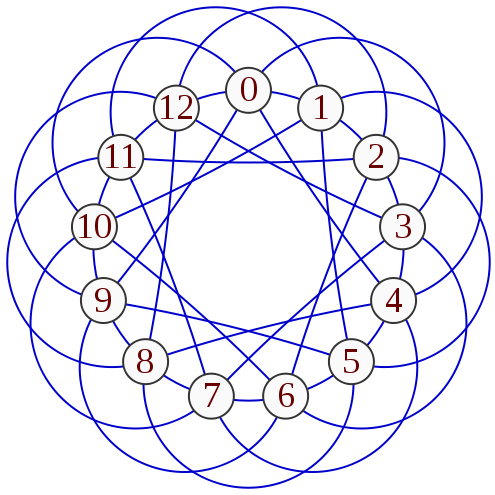
\includegraphics[scale=0.7]{srg_example.png}
    \caption{Граф Пейли 13-го порядка, сильно регулярный граф с параметрами srg(13,6,2,3).}
    \label{srg}
\end{figure}


\begin{figure}[th]
    \centering
    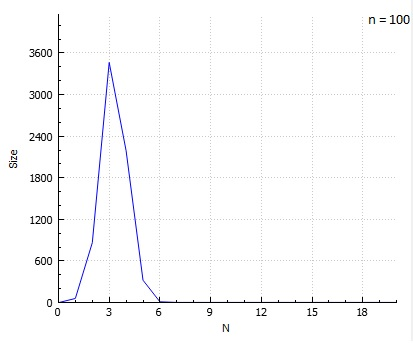
\includegraphics[]{1.jpg}
    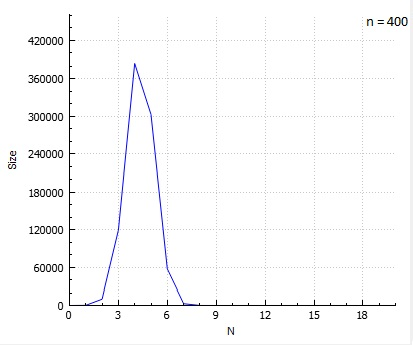
\includegraphics[]{2.jpg}
    \caption{Построение $\{ |M_m|\} $}
    \label{program_example}
\end{figure}


\section*{Приложение Б}
\addcontentsline{toc}{section}{Приложение Б}
\label{sec:Apendix_2} \index{Apendix_2}
\large

Ссылка на дипломную работу с программой на github: \ref{https://github.com/fullincome/university}

\subsection*{Б1 Листинг программного кода на фреймворке QT}
\addcontentsline{toc}{subsection}{Б1 Листинг программного кода на фреймворке QT}

\subsection*{Б2 Листинг программного кода на С++ для суперкомпьютера}
\addcontentsline{toc}{subsection}{Б2 Листинг программного кода на С++ для суперкомпьютера}